\documentclass{theme/uniprthesis}

%%%%%%%%%%%Some Extra Packages%%%%%%%%%%%
\usepackage[italian]{babel}		% To have Italina names in Sections, Figures, Chapters etc.
\usepackage{todonotes}			% To ease the revision
\usepackage{subcaption}



%%%%% THESIS / TITLE PAGE INFORMATION
% Everybody needs to complete the following:

\title{Addestramento di una rete neurale encoder-decoder con dati limitati per la segmentazione del femore fetale da immagini ecografiche}
\author{Dmitri Ollari Ischimji}
\advisor{Prof. Claudio Ferrari}
\college{Dipartimento di Ingegneria e Architettura}
\degree{Corso di Laurea Triennale in Ingegneria dei Sistemi Informativi}
\degreeyears{2023--2024}


% Not mandatory fields
\newcommand{\subTitle}{Training an encoder-decoder neural network with limited data for fetal femur segmentation from echographic images} %Subtitle, usually the english version of the title

%\newcommand{\advisorSecond}{Prof. Nome2 Cognome2} % For multiple (up to 4) advisors -- if this is not present then also the remaining ones are automatically omitted
%\newcommand{\advisorThird}{Dott. Nome3 Cognome3} % For multiple (up to 4) advisors -- if this is not present then also the remaining ones are automatically omitted
%\newcommand{\advisorFourth}{Dott. Nome4 Cognome4} % For multiple (up to 4) advisors

% \newcommand{\coadvisor}{Prof. co-Nome co-Cognome} %For multiple (up to 4) coadvisors -- if this is not present then also the remaining ones are automatically omitted
% \newcommand{\coadvisorSecond}{Prof. co-Nome2 co-Cognome2} % For multiple (up to 4) coadvisors -- if this is not present then also the remaining ones are automatically omitted
%\newcommand{\coadvisorThird}{Dott. co-Nome3 co-Cognome3} % For multiple (up to 4) coadvisors -- if this is not present then also the remaining ones are automatically omitted
%\newcommand{\coadvisorFourth}{Dott. co-Nome4 co-Cognome4} % For multiple (up to 4) coadvisors


\begin{document}

\maketitle

%%%% La dedica
\newpage
\thispagestyle{empty}
\null\vspace{\stretch{1}}
\begin{flushright}
	\textit{Dedicato a Diego}
\end{flushright}
\vspace{\stretch{3}}\null
\newpage

%%%% Gli indici
\pagestyle{plain}
\pagenumbering{arabic}
\tableofcontents
%
\listoffigures    %Commentare se non vi sono Immagini
% \listofalgorithms %Commentare se non vi sono Algoritmi
\listoftables     %Commentare se non vi sono Tabelle
%
%
%
%%%% La prefazione
% \include{Capitoli/Introduzione}
\chapter{Introduzione}
\label{chap:Introduzione}


La segmentazione semantica gioca un ruolo cruciale nell'analisi delle immagini
mediche, consentendo di identificare e isolare strutture anatomiche di
interesse. Questa tesi si concentra sull'applicazione di reti neurali
convoluzionali (CNN), in particolare sull'utilizzo dell'architettura U-Net per
la segmentazione binaria di immagini ecografiche fetali, allo scopo di estrarre
e delineare i femori.


Le immagini ecografiche fetali rappresentano una sfida complessa nella
segmentazione, richiedendo un'accurata identificazione delle strutture
anatomiche. La segmentazione semantica binaria mira all'etichettatura
specifica di pixel associati ai femori, fornendo una comprensione dettagliata
delle strutture anatomiche esaminate.

L'approccio di questa tesi si basa sull'uso della rete neurale convoluzionale
U-Net, nota per la sua efficacia nella segmentazione di immagini biomediche. La
peculiarità di U-Net è la sua capacità di catturare dettagli locali pur
mantenendo una visione globale dell'immagine, rendendola particolarmente adatta
per la segmentazione dettagliata, come l'estrazione dei femori dalle ecografie
fetali.

Attraverso l'analisi, l'implementazione e l'ottimizzazione di questa
architettura, il lavoro mira a migliorare l'accuratezza e l'efficienza della
segmentazione, fornendo uno strumento affidabile per l'identificazione
automatica dei femori nelle immagini ecografiche fetali. L'obiettivo è di
apportare un contributo significativo all'avanzamento delle tecnologie di
estrazione delle informazioni dalle immagini ecografiche, automatizzando e
facilitando una valutazione più precisa della densità minerale ossea fetale
(BMD).


%
%%%% I Capitoli di Contenuto	
\pagestyle{fancy}
  \chapter{Lavori correlati} \label{chap:related_works}
\section{Segmentazione} \label{sec:segmentazione}

\begin{figure}[!ht]
	\begin{center}
		\includegraphics[width=0.4\textwidth]{Immagini/segmantion_example_image.png}
		\includegraphics[width=0.4\textwidth]{Immagini/segmantion_example_mask.png}
	\end{center}
	\caption{Segmentazione semantica}
	\label{fig:segmentazione}
\end{figure}

La segmentazione semantica rappresenta un campo di grande interesse e rilevanza
nell'ambito dell'elaborazione delle immagini e della visione artificiale.
Questa tecnica si distingue per la sua capacità d'interpretare il contenuto
delle immagini a un livello semantico, andando oltre la semplice divisione
dell'immagine in regioni omogenee basate su caratteristiche visive come il
colore o la texture. Nello specifico, la segmentazione semantica si prefigge
l'obiettivo di attribuire un' etichetta semantica a ogni singolo pixel
dell'immagine, consentendo così d'identificare e categorizzare le diverse parti
che compongono la scena.  L'obiettivo principale della segmentazione semantica
è quello di fornire una comprensione approfondita del contenuto visivo presente
in un'immagine. Ciò si traduce nella capacità d'identificare e categorizzare
oggetti e regioni, rendendo possibile un'analisi dettagliata e una migliore
interpretazione dei dati visivi. Un esempio di applicazione della segmentazione
semantica la si pu\`o visionare nella figura \ref{fig:segmentazione}, in questo
caso l'obiettivo della segmentazione era quello di estrapolare le informazioni
relative al motociclista in una classe e le informazioni relative al veicolo in
un'altra classe, separando entrambe le classi dallo sfondo.


\section{Fully Convolutional Network}
\begin{figure}[!ht]
	\begin{center}
		\includegraphics[width=0.8\textwidth]{Immagini/cnn.png}
	\end{center}
	\caption{CNN}
	\label{fig:cnn}
\end{figure}



% \label{sec:fcn}

L'articolo \textit{Fully Convolutional Networks for Semantic Segmentation} \\
\cite{long2015fully} propone l'utilizzo di una tipologia di reti neurali
convoluzionali (CNN) che permettono grazie all'assenza di layer completamente
connessi di elaborare immagini di qualunque dimensione. Questa nuova tipologia
di reti migliora notevolmente le capacità di apprendimento delle reti neurali
permettendo di produrre mappe di segmentazione più precise grazie alla loro
capacità di apprendimento d' informazioni spaziali.

Le motivazioni per l'ampio utilizzo di queste reti nel settore della \textit{computer vision}
risiedono nell'assenza di strati completamente connessi, che solitamente vincolano l'ingresso a
dimensioni fisse per ogni immagine. Questa caratteristica permette alle reti di elaborare l'intera
immagine anziché solo frammenti, potenziando così l'apprendimento spaziale.

La maggiore flessibilità offerta da queste reti si traduce in un addestramento meno vincolato da
limitazioni dimensionali dell'input, risultando in una maggiore tolleranza agli errori e al rumore.
Di conseguenza, questa tipologia di reti si rivela particolarmente adatta in contesti caratterizzati
da una scarsità di dati.


\section{U-Net: Convolutional Networks for Biomedical Image Segmentation}

\begin{figure}[!ht]
	\begin{center}
		\includegraphics[width=0.8\textwidth]{Immagini/unet.png}
	\end{center}
	\caption{U-Net}\label{fig:unet}
\end{figure}


Nel 2015, Olaf Ronneberger, Philipp Fischer e Thomas Brox hanno introdotto il modello di rete
neurale convoluzionale \textit{U-Net} per la segmentazione semantica di immagini biomedicali
\cite{ronneberger2015unet}. Progettata specificatamente per affrontare le sfide della segmentazione
in ambito biomedico, come la necessità di segmentare con precisione strutture anatomiche con un
numero limitato di immagini di addestramento, U-Net ha rappresentato un notevole avanzamento.

Il modello \textit{U-Net} si distingue per una struttura simmetrica, dove la parte contrattiva
(downsampling) cattura il contesto e quella espansiva (upsampling) permette una localizzazione
precisa. Questa configurazione consente alla rete di fondere informazioni di contesto con quelle
locali, migliorando significativamente la precisione della segmentazione.

Grazie a queste caratteristiche, il modello \textit{U-Net} ha ottenuto risultati eccellenti nella
segmentazione di immagini biomedicali, anche con un numero limitato di immagini di addestramento,
diventando così un punto di riferimento nella segmentazione semantica biomedica.



\section{Segmentazione ossea} \label{sec:segmentazione_ossea}

Il lavoro \textit{Towards whole-body CT Bone Segmentation} \cite{10.1007/978-3-662-56537-7_59}
rappresenta un'importante analisi nello sviluppo di metodi e algoritmi avanzati per la segmentazione
ossea in immagini ottenute tramite tomografia computerizzata (TC) di tutto il corpo. Questo studio
pone l'accento sull'importanza della segmentazione ossea in campo medico, sia per la diagnosi di
condizioni patologiche sia per analisi dettagliate del tessuto osseo.

Il contributo fondamentale dell'articolo risiede nell'esplorazione di approcci innovativi e
nell'ottimizzazione di tecniche algoritmiche per identificare e isolare con precisione le strutture
ossee nelle immagini TC. Viene sottolineata l'importanza dell'uso di metodologie avanzate
nell'elaborazione delle immagini e dell'applicazione di algoritmi di visione artificiale e machine
learning per ottenere una segmentazione accurata.

L'articolo assume un ruolo significativo nel campo dell'informatica medica, evidenziando l'impiego
di soluzioni informatiche per un'analisi approfondita delle immagini mediche e riconoscendo
l'importanza delle tecniche di segmentazione ossea per applicazioni cliniche e di ricerca biomedica.


\section{Segmentazione di vasi sanguigni} \label{sec:segmentazione_vasi_sanguigni}

L'articolo \textit{Accurate Retinal Vessel Segmentation via Octave Convolution Neural Network}
\cite{fan2020accurate} introduce un approccio innovativo per la segmentazione precisa dei vasi
sanguigni retinici utilizzando le reti neurali a convoluzione ottava. Questa tecnica gioca un ruolo
cruciale nell'analisi delle immagini retiniche in ambito medico.

Il lavoro mette in luce i vantaggi offerti dalle reti neurali a convoluzione ottava, che utilizzano
differenti frequenze spaziali per catturare dettagli a diverse scale. Questo approccio risulta
particolarmente efficace nella segmentazione dei vasi sanguigni retinici, contribuendo
significativamente alla comprensione e diagnosi delle patologie oculari.

L'articolo dimostra l'efficacia di queste reti nel rilevare e isolare i vasi sanguigni della retina,
mostrando risultati più accurati rispetto ai metodi tradizionali. In definitiva, \textit{Accurate
	Retinal Vessel Segmentation via Octave Convolution Neural Network} offre un contributo importante
nel campo della segmentazione vascolare retinica, sottolineando l'efficacia e l'importanza delle
reti neurali a convoluzione ottava nella diagnostica medica.

  \chapter{Metodi} % (fold)
\label{cha:Metodi}

Tutti i dati sono stati raccolti da analisi ecografiche effettuate presso l'\textbf{Azienda
Ospedaliera Universitaria di Parma}, nel periodo tra \textbf{Aprile 2022} e \textbf{Gennaio 2023} da
un team di \textbf{medici esperti}. Per standardizzare le immagini raccolte, sono stati applicati i
seguenti parametri:

\begin{itemize}
    \item Indice di massa corporea (BMI)
    \item Età
    \item Problematiche durante la gravidanza
    \item Problematiche dopo la gravidanza
    \item Femore centrato nell'inquadratura
\end{itemize}

Le immagini sono state sottoposte a un processo di \textit{preprocessing} per uniformare dimensioni
e risoluzione, ridimensionandole a \textbf{$1280px$ di larghezza} e \textbf{$876px$ di altezza}.
Inoltre, considerando che il problema appartiene alla classe di problemi di segmentazione semantica
binaria, le immagini sono state convertite da \textbf{RGB} a \textbf{scala di grigi} per ridurre la
complessità e il quantitativo di dati necessari per l'addestramento della rete.

Per ogni immagine, sono state create manualmente delle \textbf{maschere} di segmentazione, fornendo
un \textit{ground truth} da confrontare con le predizioni del modello. Data la limitata quantità di
dati disponibili per l'addestramento della U-Net, si è ricorsi a tecniche di \textit{data
augmentation}, applicate casualmente a ogni coppia \textbf{immagine-maschera}, per aumentare la
quantità di dati. Le tecniche utilizzate includono:

\begin{itemize}
    \item \textit{Flip} orizzontale e verticale
    \item \textit{Rotazioni} di $35^{\circ}$
    \item \textit{Rumore} Gaussiano
\end{itemize}

Queste tecniche hanno migliorato notevolmente le segmentazioni ottenute tramite la rete U-Net,
aumentando la robustezza della rete alle variazioni di luce e al rumore nelle immagini.

\begin{figure}
    \centering
    \includegraphics[width=0.8\textwidth]{Immagini/data_augmentation_train.png}
    \caption{Immagini utilizzate per l'addestramento}
    \label{fig:data_augmentation_train}
\end{figure}

L'efficacia della \textit{data augmentation} nella fase di addestramento del modello è evidente,
migliorando l'adattabilità a contesti non controllati e la generalizzazione del modello. Come
mostrato in \autoref{fig:data_augmentation_train}, la \textit{data augmentation} è stata applicata in modo
casuale per ogni coppia \textbf{immagine-maschera} solo durante l'addestramento, mantenendo
inalterate le immagini usate per il controllo del modello.

Soltanto le immagini utilizzate per l'addestramento sono state sottoposte a \textit{data augmentation},
le immagini contenute nel \textit{test set} e nel \textit{validation set} sono rimaste invariate.


\begin{figure}
    \centering
    \includegraphics[width=0.8\textwidth]{Immagini/data_augmentation_test.png}
    \caption{Immagini utilizzate nel test set}
    \label{fig:data_augmentation_test}
\end{figure}

\begin{figure}
    \centering
    \includegraphics[width=0.8\textwidth]{Immagini/data_augmentation_val.png}
    \caption{Immagini utilizzate nel validation set}
    \label{fig:data_augmentation_val}
\end{figure}

È fondamentale che i set di test e validazione riflettano accuratamente le condizioni reali di
utilizzo, per valutare efficacemente le prestazioni del modello. L'introduzione di variazioni
artificiali tramite data augmentation in questi set potrebbe portare a una valutazione distorta
delle capacità del modello.

Applicare la data augmentation ai set di test e validazione potrebbe risultare in una valutazione
imprecisa delle prestazioni del modello, fornendo un'immagine ottimistica ma non realistica della
sua capacità di generalizzare su dati non modificati.

Mentre la data augmentation durante l'addestramento espone la rete a una varietà maggiore di dati, è
essenziale valutare la rete su dati non alterati per assicurarsi che abbia imparato a generalizzare
correttamente.



\section{Etichettatura}
Le immagini utilizzate per l'addestramento della rete sono state etichettate manualmente utilizzando
un software di etichettatura chiamato \textbf{LabelMe} \cite{labelme}.

Il processo di etichettatura comporta la selezione accurata e la delimitazione del perimetro del
femore in ciascuna immagine. Sono applicato indicatori specifici attorno alla regione di interesse,
in modo da isolare il femore dal resto dell'immagine. Questo approccio di etichettatura mirata è
cruciale per fornire alla rete neurale esempi precisi da cui imparare, migliorando così la sua
capacità di identificare correttamente le strutture anatomiche nelle immagini.

La corretta etichettatura è vitale non solo per l'addestramento efficace della rete, ma anche per
garantire l'affidabilità e l'accuratezza delle segmentazioni future. Essa permette alla rete di
riconoscere le variazioni sottili e le caratteristiche specifiche del femore, che sono essenziali
per applicazioni mediche precise e affidabili.




\section{Modello}

Il modello scelto come punto di partenza per questo studio è il \textbf{U-Net} (\autoref{fig:unet}),
la cui architettura originale è stata sviluppata da Olaf Ronneberger, Philipp Fischer e Thomas Brox
nel 2015 \cite{ronneberger2015unet}. Questo studio propone un'architettura di rete neurale
convoluzionale specificamente progettata per la segmentazione semantica di immagini biomediche, in
cui ogni singolo pixel dell'immagine è classificato in una delle categorie pertinenti al problema
analizzato.

La rete convoluzionale derivata da questo studio rimane una delle più impiegate nel settore medico
per la segmentazione semantica, grazie alle sue notevoli prestazioni e versatilità.
L'implementazione iniziale di questo studio si basa fedelmente sul modello proposto da Ronneberger,
Fischer e Brox, utilizzando il framework \textbf{PyTorch} \cite{pytorch} come piattaforma per lo
sviluppo della rete.


\section{Architettura U-Net}

L'architettura proposta da Olaf Ronneberger, Philipp Fischer e Thomas Brox è composta da quattro
parti principali: 
\begin{itemize} 
    \item \textbf{Encoder}: Visionabile graficamente come la parte discendente della U-Net.
    \item \textbf{Bridge}: Visionabile graficamente come la linea di congiunzione tra la parte
        discendente e quella ascendente della U-Net.
    \item \textbf{Decoder}: Visionabile graficamente come la parte ascendente della U-Net.
    \item \textbf{Output}: Visionabile graficamente come l'ultimo layer della U-Net.
\end{itemize}

Le applicazioni basate su modelli derivati dall'architettura U-Net sono ampiamente utilizzate in settori come la medicina e la biologia, particolarmente nella segmentazione di immagini biomediche, come le immagini ecografiche, TC e RM.

I motivi principali del successo di U-Net includono:
\begin{itemize} 
    \item \textbf{Segmentazione dettagliata}: U-Net è capace di produrre segmentazioni dettagliate e
        precise grazie alle sue innovative "skip connections", che consentono al modello di
        catturare sia i dettagli di basso livello che il contesto di alto livello.
    \item \textbf{Architettura compatta}: Nonostante la sua elevata capacità di dettaglio, il
        modello rimane relativamente snello e può essere addestrato con successo anche con dataset
        di dimensioni moderate.
    \item \textbf{Adattabilità}: Originariamente concepita per applicazioni mediche, U-Net ha
        dimostrato un'elevata versatilità, adattandosi a una vasta gamma di applicazioni.
\end{itemize}

Tuttavia, come ogni modello, U-Net presenta anche alcuni svantaggi. Il principale riguarda la
necessità di un dataset di addestramento ampio e accuratamente etichettato, che può essere un
ostacolo in contesti con dati limitati. Inoltre, U-Net richiede una quantità significativa di
memoria per memorizzare i pesi del modello, il che può rappresentare un problema nel caso di
immagini ad alta risoluzione.


\subsection{Convoluzione}
\label{sec:convoluzione}

La convoluzione è una delle operazioni fondamentali utilizzate nelle reti neurali convoluzionali
(CNN) per estrarre le caratteristiche significative da un'input. Essa impiega un filtro (o kernel)
che viene applicato sull'input.

Il processo di convoluzione consiste nel sommare ogni elemento di un'immagine con i suoi vicini,
pesando ogni operazione mediante l'utilizzo del filtro. La feature map di uscita viene calcolata
come segue:
\begin{align}
  &\Bigg( \begin{bmatrix}
    a & b & c \\
    d & e & f \\
    g & h & i
  \end{bmatrix}
  *
  \begin{bmatrix}
    1 & 2 & 3 \\
    4 & 5 & 6 \\
    7 & 8 & 9
  \end{bmatrix}
  \Bigg) [2, 2] =\\
  &= (i \cdot 1) + (h \cdot 2) + (g \cdot 3) + (f \cdot 4) + (e \cdot 5) + (d \cdot 6) + (c \cdot 7) + (b \cdot 8) + (a \cdot 9)
\end{align}


\subsection{Max Pooling}
\label{sec:max_pooling}

Il \textit{max pooling} è un'operazione chiave all'interno delle reti neurali convoluzionali (CNN),
inclusa la rete U-Net.

Questa tecnica è utilizzata per ridurre la dimensione delle feature map, contribuendo a diminuire la
complessità computazionale del problema. Il \textit{max pooling} aumenta la resistenza della rete
all'\textit{overfitting}, migliora la capacità di generalizzazione del modello e consente di
ottenere una rappresentazione più invariante rispetto alle piccole variazioni spaziali nell'input.


\subsection{Encoder}
\label{sec:Encoder}

La fase di \textit{encoding} rappresenta la prima parte della rete U-Net, ed è composta da una serie
di strati di convoluzione (vedi Sezione \ref{sec:convoluzione}) e max pooling (vedi Sezione
\ref{sec:max_pooling}). Questi strati lavorano per ridurre progressivamente la dimensione spaziale
dell'immagine, aumentando contemporaneamente il numero di canali delle \textit{features}.

Nello specifico, la fase di \textit{encoding} comprende tre componenti principali:
\begin{itemize}
  \item \textbf{Strato iniziale}: Questo strato applica diverse operazioni di convoluzione ai dati
      di input per estrarre caratteristiche di basso livello, come bordi e texture.
  \item \textbf{Downsampling}: Successivamente, si utilizzano operazioni di max pooling o
      convoluzione con un passo (stride) superiore a 1 per ridurre la dimensione delle feature map.
  \item \textbf{Strati intermedi}: Questi strati applicano ulteriori operazioni di convoluzione per
      catturare caratteristiche di complessità crescente.
\end{itemize}


\subsection{Decoder}
\label{sec:Decoder}

La fase di \textit{decoding} nella rete U-Net è incaricata di ricostruire l'immagine segmentata a
partire dalle informazioni estratte durante la fase di \textit{encoding}. Le fasi principali del
decoder includono:
\begin{itemize}
  \item \textbf{Upsampling}: Per ripristinare gradualmente la dimensione originale delle feature map.
  \item \textbf{Skip Connections}: Per combinare informazioni multi-scala.
  \item \textbf{Convoluzione nel Decoding}: Per affinare ulteriormente le feature map dopo
      l'upsampling e l'integrazione delle skip connections.
\end{itemize}

\subsection{Bridge}
\label{sec:Bridge}

Il \textit{bridge} è una componente cruciale dell'architettura U-Net, che facilita il trasferimento
di informazioni rilevanti tra l'encoder e il decoder attraverso le \textit{skip connections}. Questa fase
consente di considerare dettagli sia di basso che di alto livello durante il processo di
segmentazione.

\subsection{Output}
\label{sec:Output}
La parte finale della rete U-Net è costituita da uno o più strati di convoluzione che riducono la
profondità delle feature map alla dimensione richiesta per l'output finale, producendo così
l'immagine segmentata.


\section{Rimozione della Sliding Window}
\label{sub:Rimozione sliding window}

Con gli avanzamenti tecnologici nel campo dell'hardware e del software, si è osservato un notevole
miglioramento nei tempi di elaborazione delle immagini e nella capacità di gestire immagini di
grandi dimensioni. Pertanto, si è deciso di abbandonare l'approccio della sliding window, che è più
conservativo in termini di utilizzo della memoria e tempo di elaborazione.

Al suo posto, si è adottato un metodo più moderno che sfrutta la potenza di calcolo delle GPU
attuali e la loro memoria dedicata, significativamente più ampia rispetto alle generazioni
precedenti. L'utilizzo di immagini complete, anziché porzioni separate tramite sliding window, ha
prodotto un "effetto collaterale" positivo: una migliore comprensione spaziale delle immagini da
parte della rete.

La visualizzazione dell'intera immagine consente alla rete di acquisire una migliore comprensione
del contesto spaziale, migliorando così la precisione della segmentazione.


\section{Modifica della Struttura Encoder-Decoder}
\label{sub:Modifica Encoder-Decoder}

Durante le fasi sperimentali, è emerso che aumentando il numero di iterazioni di convoluzione nei
vari strati di encoding e decoding si ottengono risultati migliori in termini di segmentazione.
Questo miglioramento, tuttavia, comporta un aumento del tempo di elaborazione e del consumo di
memoria.

Di conseguenza, si è deciso di modificare le fasi di \textit{encoding} e \textit{decoding} come segue:

\begin{table}[!ht]
    \centering
    \begin{tabular}{|c|c|c|}
        \hline
        \textbf{Layer} & \textbf{In channels} & \textbf{Out channels} \\
        \hline
        \hline
        Encoder        & 1                    & 64                    \\
        \hline
        Encoder        & 64                   & 128                   \\
        \hline
        Encoder        & 128                  & 256                   \\
        \hline
        Encoder        & 256                  & 512                   \\
        \hline
        Decoder        & 1024                 & 512                   \\
        \hline
        Decoder        & 512                  & 256                   \\
        \hline
        Decoder        & 256                  & 128                   \\
        \hline
        Decoder        & 128                  & 64                    \\
        \hline
    \end{tabular}
    \caption{Encoding e Decoding originali}
    \label{tab:encoding_originale}
\end{table}

\begin{table}[!ht]
    \centering
    \begin{tabular}{|c|c|c|}
        \hline
        \textbf{Layer} & \textbf{In channels} & \textbf{Out channels} \\
        \hline
        \hline
        Encoder        & 1                    & 16                    \\
        \hline
        Encoder        & 16                   & 32                    \\
        \hline
        Encoder        & 32                   & 64                    \\
        \hline
        Encoder        & 64                   & 128                   \\
        \hline
        Encoder        & 128                  & 256                   \\
        \hline
        Encoder        & 256                  & 512                   \\
        \hline
        Decoder        & 1024                 & 512                   \\
        \hline
        Decoder        & 512                  & 256                   \\
        \hline
        Decoder        & 256                  & 128                   \\
        \hline
        Decoder        & 128                  & 64                    \\
        \hline
        Decoder        & 64                   & 32                    \\
        \hline
        Decoder        & 32                   & 16                    \\
        \hline
    \end{tabular}
    \caption{Encoding e Decoding modificati}
    \label{tab:encoding_modificato}
\end{table}

L'intento di questa modifica è sfruttare la capacità di estrazione di feature delle operazioni di
convoluzione e di riduzione delle feature meno rilevanti tramite max pooling. Aggiungendo iterazioni
di convoluzioni, la rete può estrarre più feature importanti per la classificazione dei pixel,
mentre il max pooling aiuta a eliminare le feature meno significative, riducendo la dimensione delle
feature map.

% section Modifica Encoder-Decoder (end)


\section{Metriche}
\label{sec:metriche}

Per valutare le prestazioni del modello nel contesto del task di segmentazione, si è scelto di
utilizzare la metrica \textit{Dice BCE Loss} per la funzione di perdita e \textit{Intersection over
Union (IoU)} per misurare l'accuratezza.

\subsection{Dice BCE Loss}
\begin{figure}[!ht]
  \centering
  \includegraphics[width=0.7\columnwidth]{Immagini/dice_loss.png}
  \caption{Rappresentazione della Dice Loss}
  \label{fig:dice_loss}
\end{figure}

La \textit{Dice Loss} è una funzione di perdita basata sul coefficiente di Dice, che misura la
somiglianza tra due campioni. Questa metrica è particolarmente utile in contesti dove la regione di
interesse occupa una porzione limitata dell'immagine, come spesso accade nelle immagini mediche. Il
coefficiente di Dice è definito come segue:

La \textit{Binary Cross-Entropy (BCE) Loss} è ampiamente usata nei problemi di classificazione
binaria, specialmente quando i dati di output sono probabilità che variano tra 0 e 1. Questa metrica
valuta quanto le predizioni del modello si discostino dai valori reali (etichette).

\begin{align}
    L & = L_{\text{Dice}} + L_{\text{BCE}}
    \label{eq:dice_bce_loss}
\end{align}

\begin{align}
    L_{\text{Dice}} & = 1 - \frac{2\sum_i^N p_i g_i + \varepsilon}{\sum_i^N p_i^2 + \sum_i^N g_i^2 + \varepsilon}
    \label{eq:dice_loss}
\end{align}

\begin{align}
    L_{\text{BCE}} & = -\frac{1}{N} \Bigg[ \sum_{i=1}^N g_i \log(p_i) + (1 - g_i) \log(1 - p_i) \Bigg]
    \label{eq:bce_loss}
\end{align}

Dunque, la \textit{loss} totale viene calcolata mediante:
\begin{align}
    L & = 1 - \frac{2\sum_i^N p_i g_i + \varepsilon}{\sum_i^N p_i^2 + \sum_i^N g_i^2 + \varepsilon} -\frac{1}{N} \Bigg[ \sum_{i=1}^N g_i \log(p_i) + (1 - g_i) \log(1 - p_i) \Bigg]
    \label{eq:dice_bce_loss_complete}
\end{align}
Dove:
\begin{itemize}
    \item $p_i$ rappresenta la probabilità predetta dal modello per il pixel $i$.
    \item $g_i$ è il valore di \textit{ground truth} per il pixel $i$.
\end{itemize}


\subsection{Intersection over Union (IoU)}
\label{subsec:intersection_over_union}

Per valutare l'accuratezza della segmentazione, è stata impiegata la metrica \textit{Intersection
over Union} (IoU), che è un indicatore efficace della capacità di segmentazione del modello. L'IoU
calcola il rapporto tra l'area di intersezione e l'area di unione delle maschere predette e di
\textit{ground truth}. La formula è la seguente:
\begin{align}
    \text{IoU} & = \frac{\text{TP}}{\text{TP} + \text{FP} + \text{FN}}
    \label{eq:iou}
\end{align}
Dove \textbf{TP} rappresenta i \textit{True Positive}, \textbf{FP} i \textit{False Positive}, e
\textbf{FN} i \textit{False Negative}.


\section{Validazione del Modello}
\label{sec:model_validation}

La \textit{cross-validation} (validazione incrociata) è un metodo essenziale nel machine learning
per valutare le prestazioni di un modello in modo robusto. Questa tecnica comporta la valutazione
del modello su più insiemi di dati per ottenere stime più affidabili delle sue capacità predittive,
contribuendo a mitigare il rischio di overfitting.

\begin{figure}[!ht]
    \centering
    \includegraphics[width=0.7\textwidth]{Immagini/cross_validation.png}
    \caption{Rappresentazione grafica della Cross-validation}
    \label{fig:cross_validation}
\end{figure}

La cross-validation fornisce stime più affidabili delle prestazioni del modello, riducendo il
rischio che le valutazioni delle prestazioni siano influenzate da una singola suddivisione dei dati.

  \chapter{Risultati sperimentali} % (fold)
\label{chap:Risultati sperimentali}

\section{Addestramento} % (fold)
\label{sec:Addestramento}

Il modello \`e stato addestrato mediante l'uso della \textit{cross-validation}(\autoref{fig:cross_validation})
con una suddivisione dei dati in cinque parti uguali(cinque folds).

Essendo una tipologia di apprendimento supervisionata, al modello sono fornite immagini
originali e le loro segmentazioni effettuate manualmente.

\begin{figure}[!ht]
    \centering
    \includegraphics[width=0.7\columnwidth]{Immagini/training.png}
    \caption{Addestramento del modello}
    \label{fig:addestramento del modello}
\end{figure}


Effettuando l'addestramento con 5 folds, il modello viene addestrato 5 volte, ogni volta con un fold diverso,
l'errore finale \`e dato dalla media degli errori ottenuti dalle 5 iterazioni.

\begin{figure}[!ht]
    \centering
    \includegraphics[width=0.4\columnwidth]{Immagini/fold_0_loss.png} \includegraphics[width=0.4\columnwidth]{Immagini/fold_0_accuracy.png}
    \caption{Errore e accuratezza della prima porzione di dati}
    \label{fig:loss e accuratezza della prima porzione di dati}
\end{figure}

\begin{figure}
    \centering
    \includegraphics[width=0.4\columnwidth]{Immagini/fold_1_loss.png} \includegraphics[width=0.4\columnwidth]{Immagini/fold_1_accuracy.png}
    \caption{Errore e accuratezza della seconda porzione di dati}
    \label{fig:loss e accuratezza della seconda porzione di dati}
\end{figure}

\begin{figure}
    \centering
    \includegraphics[width=0.4\columnwidth]{Immagini/fold_2_loss.png} \includegraphics[width=0.4\columnwidth]{Immagini/fold_2_accuracy.png}
    \caption{Errore e accuratezza della terza porzione di dati}
    \label{fig:loss e accuratezza della terza porzione di dati}
\end{figure}

\begin{figure}
    \centering
    \includegraphics[width=0.4\columnwidth]{Immagini/fold_3_loss.png} \includegraphics[width=0.4\columnwidth]{Immagini/fold_3_accuracy.png}
    \caption{Errore e accuratezza della quarta porzione di dati}
    \label{fig:loss e accuratezza della quarta porzione di dati}
\end{figure}

\begin{figure}
    \centering
    \includegraphics[width=0.4\columnwidth]{Immagini/fold_4_loss.png} \includegraphics[width=0.4\columnwidth]{Immagini/fold_4_accuracy.png}
    \caption{Errore e accuratezza della quinta porzione di dati}
    \label{fig:loss e accuratezza della quinta porzione di dati}
\end{figure}

L'\textbf{errore} complessivo viene calcolato come media dei singoli errori
ottenuti dalle cinque iterazioni mediante la formula
\ref{eq:dice_bce_loss_complete} portando a un errore medio del
\textbf{$7.9\%$}.

Mentre l'\textbf{accuratezza} complessiva viene calcolata come media delle singole accuratezze
ottenute dalle cinque iterazioni mediante la formula \ref{eq:iou} portando a un'accuratezza media del \textbf{$92.1\%$}.




Considerando che questo modello \`e stato utilizzato in ambito medico per velocizzare e standardizzare 
la segmentazione dei femori per un'analisi su questi ultimi, oltre ad analisi quantitative, \`e stato 
necessario effettuare delle analisi qualitative sulla segmentazione ottenuta dal modello.

Nelle immagini seguenti viene riportato uno delle immagini prese in considerazione per l'addestramento del modello
e vengono mostrate le segmentazione manuali, le segmentazioni ottenute dal modello e la differenze 
nella classificazione dei pixel tra le due segmentazioni.





Partendo da una immagini (\autoref{fig:immagine originale}) ottenuta mediante la raccolta dati effettuata dai medici, 

\begin{figure}[!ht]
    \centering
    \includegraphics[width=0.7\columnwidth]{Immagini/image.png}
    \caption{Immagine originale}
    \label{fig:immagine originale}
\end{figure}


% I risultati ottenuti mediante la segmentazione manuale e la segmentazione del modello sono 
% rispettivamente \autoref{fig:segmentazione manuale} e \autoref{fig:segmentazione del modello}.

% \begin{figure}[!ht]
%     \centering
%     \includegraphics[width=0.4\columnwidth]{Immagini/mask.png}
%     \caption{Segmentazione manuale}
%     \label{fig:segmentazione manuale}
% \end{figure}

% \begin{figure}[!ht]
%     \centering
%     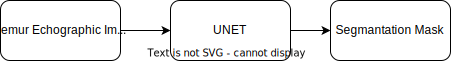
\includegraphics[width=0.4\columnwidth]{Immagini/prediction.png}
%     \caption{Segmentazione del modello}
%     \label{fig:segmentazione del modello}
% \end{figure}

\begin{figure}[!ht]
    \centering
    \begin{minipage}{0.4\columnwidth}
        \centering
        \includegraphics[width=\linewidth]{Immagini/mask.png}
        \caption{Segmentazione manuale}
        \label{fig:segmentazione manuale}
    \end{minipage}
    \hfill
    \begin{minipage}{0.4\columnwidth}
        \centering
        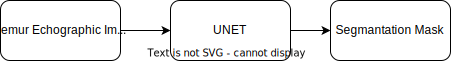
\includegraphics[width=\linewidth]{Immagini/prediction.png}
        \caption{Segmentazione del modello}
        \label{fig:segmentazione del modello}
    \end{minipage}
\end{figure}

Per sostenere la tesi che il modello riesca a segmentare correttamente le immagini, \`e stata 
calcolata la distribuzione dei pixel per confrontare la segmentazione manuale con quella del modello.

% Per quantifica la differenza tra le due segmentazioni \`e stata calcolata la distribuzione dei pixel
% nelle immagini processate manuale e si \`e confrontata con la distribuzione dei pixel nelle immagini
% processate dal modello

% \begin{figure}[!ht]
%     \centering
%     \includegraphics[width=0.7\columnwidth]{Immagini/handmade_scaled_hist.png}
%     \caption{Distribuzione Intensità dei pixel della segmentazione manuale}
%     \label{fig:distribuzione intensità dei pixel della segmentazione manuale}
% \end{figure}

% \begin{figure}[!ht]
%     \centering
%     \includegraphics[width=0.7\columnwidth]{Immagini/model_scaled_hist.png}
%     \caption{Distribuzione Intensità dei pixel della segmentazione del modello}
%     \label{fig:distribuzione intensità dei pixel della segmentazione del modello}
% \end{figure}

\begin{figure}[!ht]
    \centering
    \begin{minipage}{0.45\columnwidth}
        \centering
        \includegraphics[width=\linewidth]{Immagini/handmade_scaled_hist.png}
        \caption{Distribuzione Intensità dei pixel della segmentazione manuale}
        \label{fig:distribuzione intensità dei pixel della segmentazione manuale}
    \end{minipage}
    \hfill
    \begin{minipage}{0.45\columnwidth}
        \centering
        \includegraphics[width=\linewidth]{Immagini/model_scaled_hist.png}
        \caption{Distribuzione Intensità dei pixel della segmentazione del modello}
        \label{fig:distribuzione intensità dei pixel della segmentazione del modello}
    \end{minipage}
\end{figure}

\begin{figure}[!ht]
    \centering
    \includegraphics[width=0.7\columnwidth]{Immagini/handmade_vs_model_scaled.png}
    \caption{Confronto tra la segmentazione manuale e quella del modello}
    \label{fig:confronto tra la segmentazione manuale e quella del modello}
\end{figure}


Dai risultati qualitativi e quantitativi si pu\`o constatare che il modello ha una performance
molto promettente in quanto supera abbondantemente un'accuratezza del $90\%$ e pu\`o essere 
addestrato incrementando il numero d'immagini a disposizione. 

Non sono necessari ulteriori segmentazioni manuali ma si possono direttamente sfruttare
le nuove immagini raccolte, segmentarle mediante l'uso del modello e utilizzarle per l'addestramento.




% % section Addestramento (end)





% % chapter Risultati sperimentali (end)

\pagestyle{plain}
\chapter{Conclusioni}
\label{chap:Conclusioni}

Il modello sviluppato in questo studio è stato progettato per automatizzare la segmentazione di
immagini di femori fetali \cite{abstract1} \cite{abstract2}. L'utilizzo del modello consente di
automatizzare un compito che altrimenti richiederebbe tempo e impegno da parte di un professionista,
liberando risorse per altre attività.

Specificamente, il modello è stato impiegato per automatizzare l'estrazione dei pixel del femore di
un feto nelle settimane 35-37 di gestazione. I pixel estratti sono stati analizzati per determinare
la luminosità, che nelle ecografie è correlata alla \textbf{densità minerale ossea} (\textbf{BMD})
del femore fetale, e per studiarne la correlazione con il peso di nascita.

Una correlazione debole è stata rilevata tra la luminosità e il peso alla nascita, come illustrato
nella Figura \ref{fig:correlazione tra luminosità e peso alla nascita}.

\begin{figure}[!ht]
	\centering
	\includegraphics[width=0.6\columnwidth]{Immagini/correlation_weight_abstract.png}
	\caption{Correlazione tra luminosità e peso alla nascita}
	\label{fig:correlazione tra luminosità e peso alla nascita}
\end{figure}

La rete neurale ha dimostrato di essere efficace nel riconoscere i pixel contenenti informazioni
sull'area del femore. Inoltre, i risultati prodotti dalla rete suggeriscono la possibilità di
utilizzare questo approccio per ulteriori analisi.


I risultati dell'addestramento permettono di concludere che il modello è in grado di gestire con
efficacia set di dati diversi da quelli utilizzati per l'addestramento. Questo suggerisce un
potenziale significativo per miglioramenti attraverso un addestramento mirato, che potrebbe affinare
ulteriormente la capacità del modello di gestire con efficacia set di dati simili.

% Sottolineando il fatto che il modello non \`e specificamente addestrato su questi dati, la sua
% performance qualitativa appare accettabile. Ciò suggerisce un potenziale significativo per
% miglioramenti attraverso un addestramento mirato, che potrebbe affinare ulteriormente la capacità
% del modello di gestire con efficacia set di dati simili.
%
%

% I risultati ottenuti dal secondo ecografo hanno sottolineato la capacità del modello di generalizzare,
% il modello non è stato addestrato su questi dati e la sua performance qualitativa appare accettabile.
%
% Ciò suggerisce un potenziale significativo per miglioramenti attraverso un addestramento mirato, che
% potrebbe affinare ulteriormente la capacità del modello di gestire con efficacia set di dati simili.
%
%

Ne deriva che i punti di forza del modello sono la capacità di generalizzare
con pochi dati e su ecografi differenti, aprendo possibilità di portabilità del
modello su differenti ecografi senza necessit\`a specifica di ulteriore
addestramento specifico al macchinario.

D'altro canto come in tutte le applicazioni di deep learning, il modello
giova di una quantità di dati sufficiente per rendere il sistema robusto e
capace di generalizzare.

%
%%%% La bibliografia
\bibliographystyle{apalike} %{plain} -- Scegliere lo stile preferito
\cleardoublepage
\addcontentsline{toc}{chapter}{\bibname}
\bibliography{./Bibliografia}
%
% \include{Capitoli/Ringraziamenti}
%
% Le appendici
\appendix
% \include{Capitoli/Appendici/Appendice1}
%
\end{document}
